\section{Smart/Intelligent Windows}
Requirements\\
Tell how 

\section{Thermochromic Materials}
Materials that change their optical nature when subject to irradiation by light(photons),
temperature change or an applied electric field are called photochromic, thermochromic and 
electrochromic, respectively, and go under the gathered term chromic materials.
(\cite{Kiri2010},1)
\\
\\
The word thermochromic originates from Greek, meaning warm or hot (''Thermos'') and color (''Chroma'').
As mentioned earlier, thermochromic materials their optical properties in response to changes in
temperature and results in the material changing color (\cite{Kamalisarvestani},74,75). 
\\
\\
Typically, this change in color happens gradually over a range of temperatures. In this case it is called
continuous thermochromism. Discontinuous thermochromism also occurs and involves a structural
phase change at a certain characteristic ''transition temperature'' $T_t$ (\cite{Kiri2010}, 1). 
\\
\\
What happens is that the thermochromic material is initially in its monoclinic state (cold state), 
where it behaves as a semiconductor being less reflective especially in the near-infrared(IR) region. 
Heating (\textbf{?This is a legit word right?}) the material, it will
at a certain temperature, known as the transition temperature, change from the monoclinic state to a 
rutile state. In its rutile state (hot state) the material acts like a semi-metal, reflecting 
a wide range of solar radiation. This change of state is called metal-to-semiconductor
transition (MST) (\cite{Kamalisarvestani},76) and is fully reversible, 
\textbf{???} co-occured with large variations in 
both electrical and optical properties in the near-IR range (83). \textbf{??? -> check if understood and 
correctly written. E.g. what is co-occured?} \\
\\
(Main articles from section was based on \cite{Kamalisarvestani2013} and \cite{Kiri2010})\\



\section{Thermochromic Windows}
\begin{figure}[h!]
  \centering
   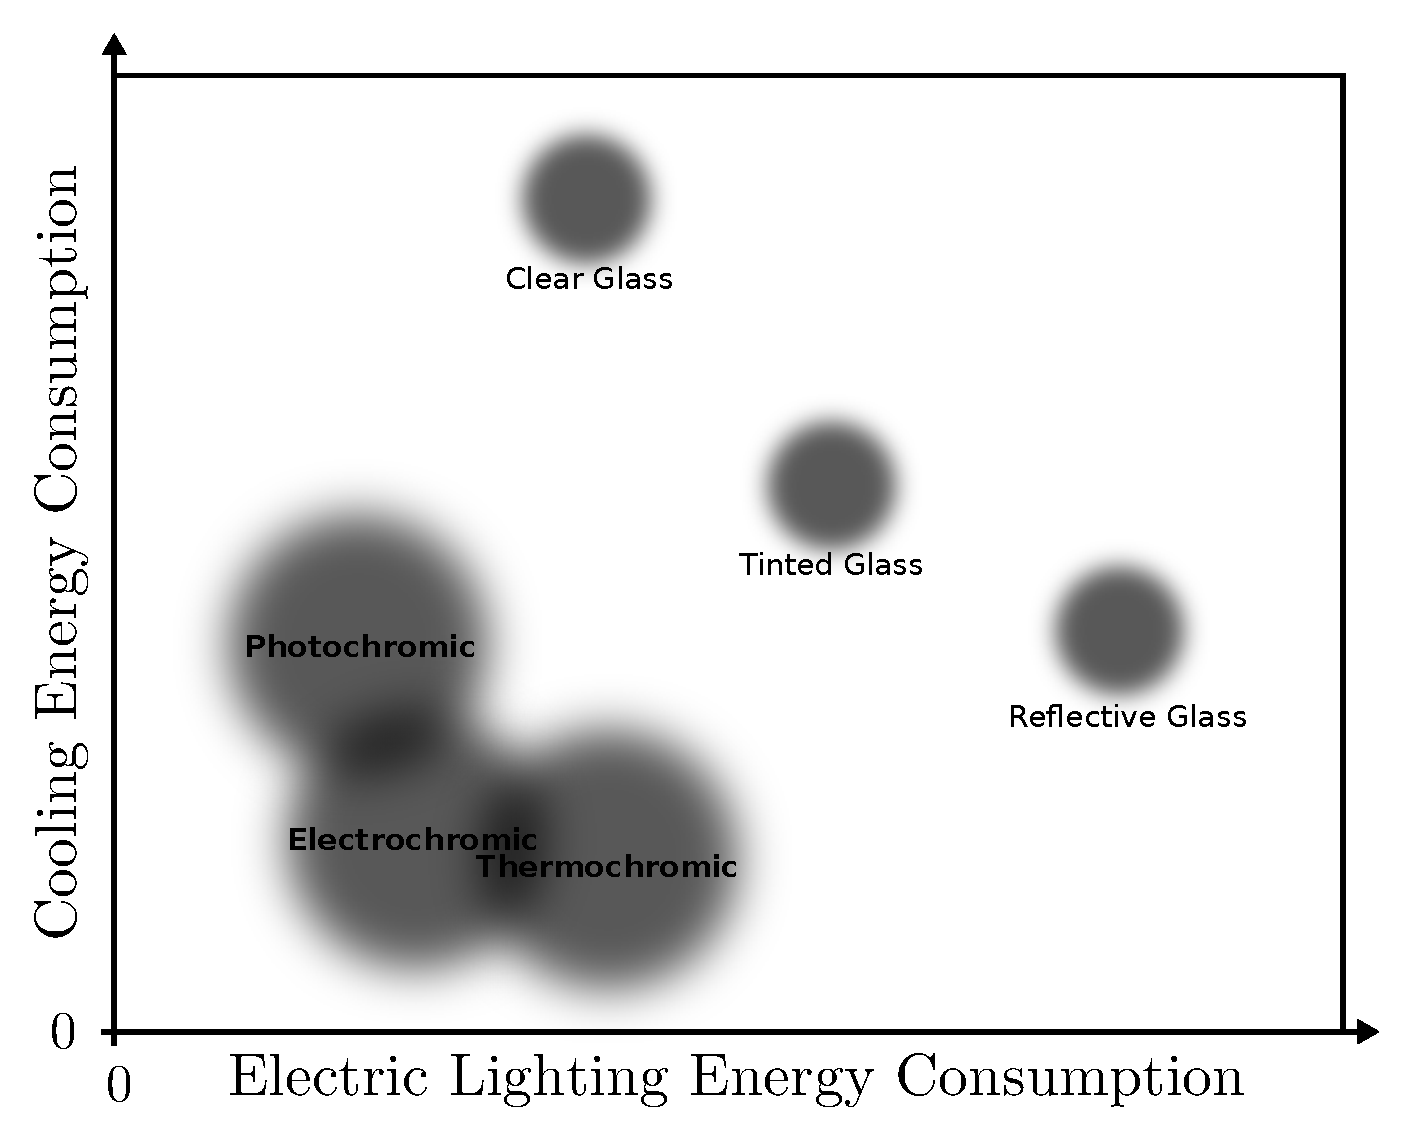
\includegraphics[width=0.5\textwidth]{Figures/chromicGlassComparison.pdf}
   \caption{Comparison of the electric lighting energy and cooling energy consumption between different
   glazing types. Adapted from (\cite{Kamalisarvestani2013},24). \textit{CHECK THIS!!: I understand
      that this graph shows the energy consumption of buildings using using different
      glazing for their windows, i.e. the window glazing impact of the building energy consumption; CHECK END.
      Also, I just drew the graph as good as I could from Kamalisarvestani2013. Is it still okay to use it?
      Should I comment on it not being exact (in case someone try to use data or something, I don't know)?}
   }
\end{figure}
%
\begin{figure}[h!]
  \centering
   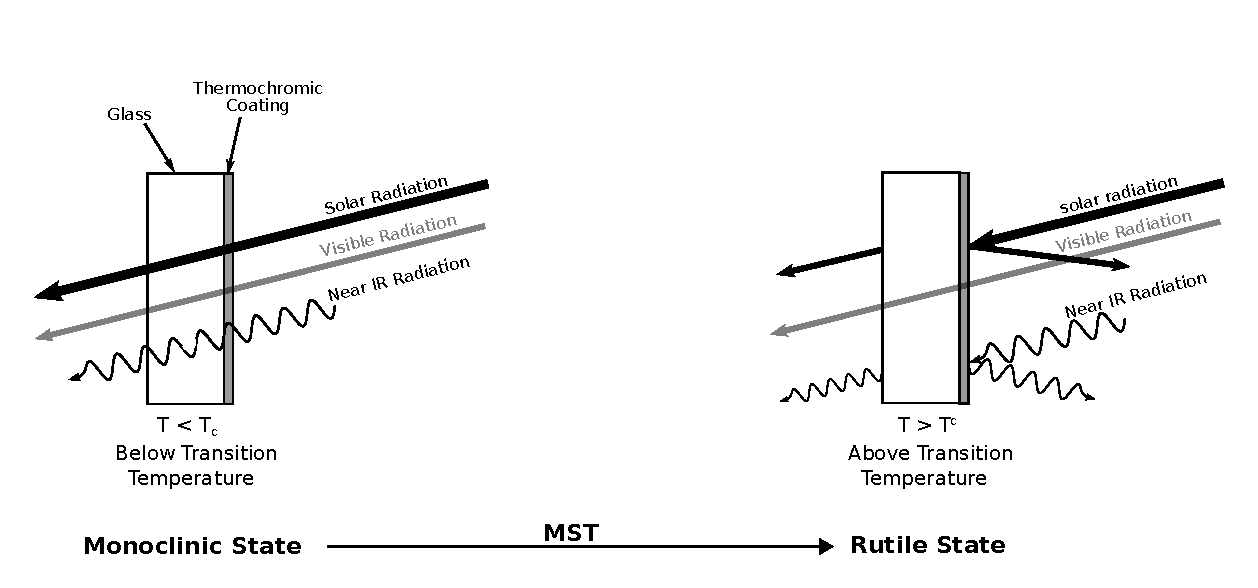
\includegraphics[width=0.9\textwidth]{Figures/TCcoating2.pdf}
   \caption{Schematic representation of thermochromic materials applied as an 
   intelligent window coating \cite{Kiria2010}.
   }
\end{figure}
%
%
\begin{figure}[h!]
  \centering
   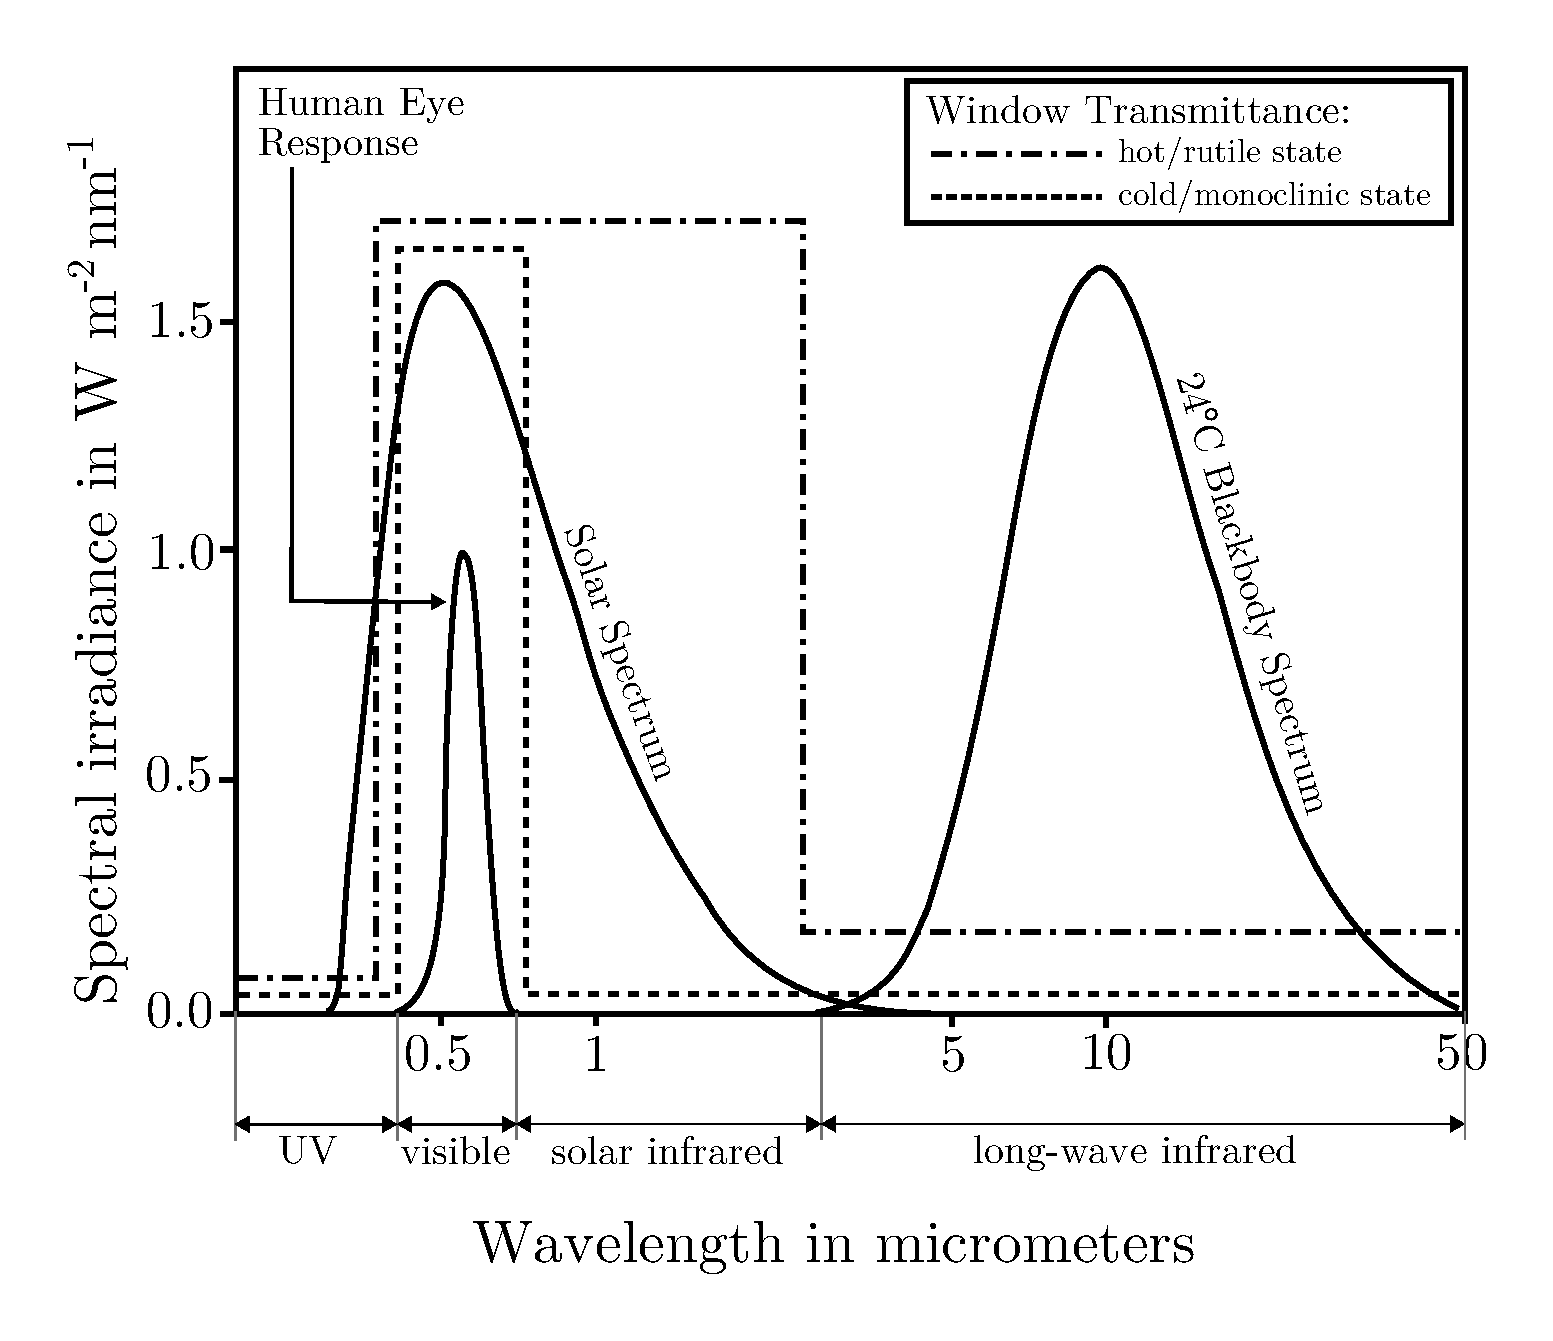
\includegraphics[width=0.5\textwidth]{Figures/TCWtransmittanceMcCluney1996andKamali2013.pdf}
   \caption{The spectral transmittance of a perfect thermochromic window, shown for both 
   cold and hot environments (the monoclinic and rutile state, repsectively). 
   Adopted from \cite{McCluney1996} \cite{Kamalisarvestani2013}
   }
\end{figure}



\textbf{Disposition:}\\
Requirements\\
- Ideal behavior- RADIATION FIGURE and PICTOGRAM\\
- ambient transition temperature\\
- 60\% transmittance in visible range, for lighting\\
-  *Doping\\
-  *Stress/strain\\
-  *thickness\\
\\
- price and mass producable: materials used and current technology\\
\\
Best Candidates:\\
(strengths and weaknesses)\\
-VO2 \\
-etc...\\


\begin{thebibliography}{9}

      \bibitem{McCluney1996}
      McCluney R, Center FSE. 
      Fenestration solar gain analysis. 
      Citeseer 1996.
      
      \bibitem{Kiri2010}
      Kiri P, Hyett G, Binions R.
      Solid state thermochromic materials.
      Advances Material Letters 2010;1(2):20.

\end{thebibliography}
